
\subsection{package edu.kit.pse.fridget.client.service}
\begin{figure}[H]
	       \centering
	       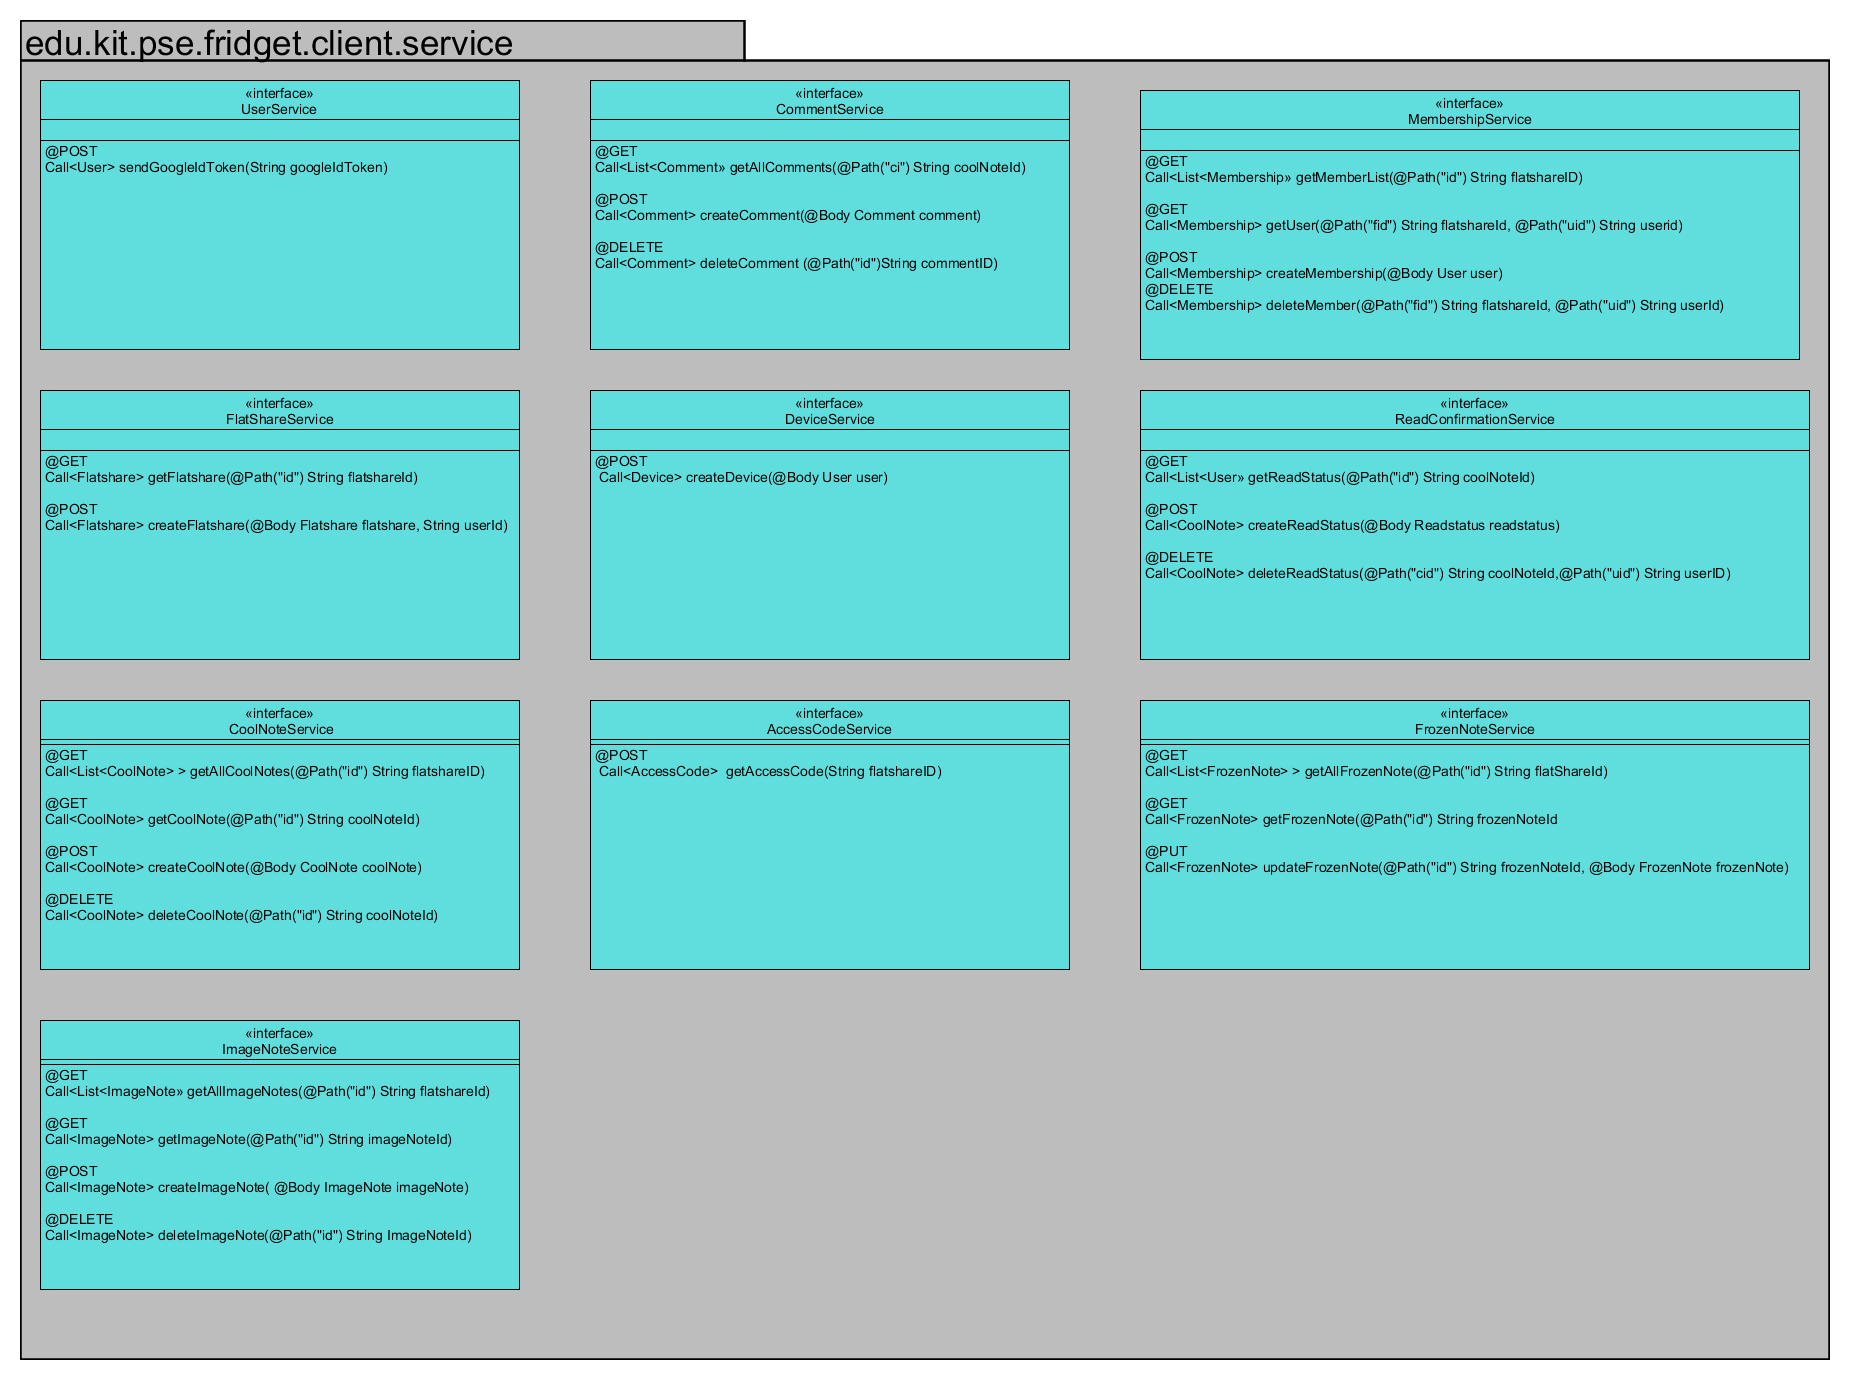
\includegraphics[scale = .26]{service.png}
	       \caption{Klassen des Services}
	      \end{figure}	
	\subsubsection{\texttt{public interface UserService}}
\textit{Dieses Interface dient dazu, den Google-Token an den Server weiterzuleiten.}\\

	\textbf{Methoden}
		\begin{itemize}

      \item\texttt{{@POST\\ Call<User> sendGoogleIdToken(String googleIdToken)}}

		\textit{Diese Methode sendet den GoogleIdToken an den Server}

		\textbf{Parameter}
		\begin{itemize}
			\item\texttt{googleIdToken}
			\textit{zu sendender GoogleToken}
		\end{itemize}
	
		\textbf{Rückgabewert}
		GoogleToken
	

	 \end{itemize}

	\subsubsection{\texttt{public interface AccessCodeService}}
\textit{Dieses Interface ist für die Synchronisation des Accesscodes mit dem Server zuständig }\\
\\
	\textbf{Methoden} \\
		\begin{itemize}
		\item{Call<AccessCode> getAccessCode(String flatShareID)}

		\textit{Diese Methode fordert den Accesscode einer Flatshare an}

		\textbf{Parameter} \\
	flatshareId - übergebende ID der Flatshare

		\textbf{Rückgabewert} \\
	Accesscode der Flatshare


	 \end{itemize}

		\subsubsection{\texttt{public interface CommentService }}
\textit{Dieses Interface ist für die Synchronisation der Comments mit dem Server zuständig}\\
\\
	\textbf{Methoden} \\
		\begin{itemize}
		\item{@GET("comments?cool-note=\{cid\}")\\ Call<List<Comment>> getAllComments(@Path(\grqq cid\grqq)String coolNoteId)}

		\textit{Diese Methode ruft alle Kommentare einer Cool Note ab}

		\textbf{Parameter} \\
	 coolNoteId - die Id der Cool Note 

		\textbf{Rückgabewert} \\
	Alle Comments der zur CoolNoteId gehörenden Cool Note


      \item{@POST("/comments")
\\ Call<Comment> createComment(@Body Comment comment)}

		\textit{Diese Methode schickt einen Comment an den Server }

		\textbf{Parameter} \\
		 comment - speichert einen Comment

		\textbf{Rückgabewert} \\
	Ein Comment

	 \item{@DELETE("/comments/{id}")\\ Call<Comment> deleteComment (@Path(\grqq id\grqq)String commentID)}

		\textit{Diese Methode löscht einen Comment }

		\textbf{Parameter} \\
		 commentID - ID des zu löschenden Comments 
		 

	 \end{itemize}


	\subsubsection{\texttt{public interface CoolNoteService }}
\textit{Dieses Interface ist für die Synchronisation der Cool Notes mit dem Server zuständig}\\
\\
	\textbf{Methoden} \\
		\begin{itemize}
		\item{@GET("/cool-notes?flatshare={id}")\\ Call<List<CoolNote>> getAllCoolNotes(@Path(\grqq id\grqq) String flatshareID)} 

		\textit{Diese Methode ruft alle Cool Notes einer Flatshare ab}

		\textbf{Parameter} \\
	flatshareId - Die Flatshare der abzurufenden Cool Notes

		\textbf{Rückgabewert} \\
	Alle Cool Notes

      \item{@GET("/cool-notes/{id}")\\ Call<CoolNote> getCoolNote(@Path(\grqq id\grqq) String coolNoteId)}

		\textit{Diese Methode ruft den Inhalt einer Cool Note ab }

		\textbf{Parameter} \\
		coolNoteId - Die Id der Cool Note 

		\textbf{Rückgabewert} \\
	Inhalt der zu der CoolNoteId gehörenden Cool Note

      \item{@POST("/cool-notes")\\ Call<CoolNote> createCoolNote(@Body CoolNote coolNote)}

		\textit{Diese Methode schickt eine neue Cool Note an den Server }

		\textbf{Parameter} \\
		coolNoteI - Die Cool Note 

		\textbf{Rückgabewert} \\
	Cool Note


      \item{@DELETE("/cool-notes/{id}")\\ Call<CoolNote> deleteCoolNote(@Path(\grqq id\grqq) String coolNoteId)}

		\textit{Diese Methode löscht eine Cool Note }

		\textbf{Parameter} \\
		coolNoteId - Die Id der Cool Note 


	 \end{itemize}


	\subsubsection{\texttt{public interface FlatShareService }}
\textit{Dieses Interface verwaltet die Synchronisation der Flatshare mit dem Server}\\
\\
	\textbf{Methoden} \\
		\begin{itemize}
		\item{@POST ("/flatshares") \\
Call<Flatshare> createFlatshare(@Body Flatshare flatshare, String userId)
}

		\textit{Diese Methode erstellt eine neue Flatshare auf dem Server
}

		\textbf{Parameter} \\
	flatshare - Name der zu erstellenden Flatshare
	userID - ID des Users, der die Flatshare erstellt

		\textbf{Rückgabewert} \\
	Flatshare

      \item{@GET("/flatshares/{id}")\\ Call<Flatshare> getFlatshare(@Path(\grqq id\grqq) 					String flatshareId)}

		\textit{Diese Methode ruft die Flatshare-Daten vom Server ab}

		\textbf{Parameter} \\
		flatshareId - die ID der aufgerufenen Flatshare 

		\textbf{Rückgabewert} \\
	Flatshare


	 \end{itemize}



	\subsubsection{\texttt{public interface FrozenNoteService }}
\textit{Dieses Interface ist für die Synchronisation der Frozen Notes mit dem Server zuständig}\\
\\
	\textbf{Methoden} \\
		\begin{itemize}
		\item{@GET("/frozen-notes?flatshare={id}")\\
Call<List<FrozenNote>> getAllFrozenNote(@Path(\grqq id\grqq) String flatShareId)}

		\textit{Diese Methode ruft die Frozen Notes vom Server ab}

		\textbf{Parameter} \\
	flatshareId -  die ID der aufgerufenen Flatshare  

		\textbf{Rückgabewert} \\
	Frozen Note

      \item{@GET("/frozen-notes/{id}")\\ Call<FrozenNote> getFrozenNote(@Path(\grqq id\grqq) String frozenNoteId)}

		\textit{Diese Methode ruft den Inhalt einer Frozen Note ab }

		\textbf{Parameter} \\
		frozenNoteId - die ID der aufgerufenen Frozen Note  

		\textbf{Rückgabewert} \\
	FrozenNote

	 \item{@PUT("/frozen-notes/{id}")\\ Call<FrozenNote> updateFrozenNote(@Path(\grqq id\grqq) String frozenNoteId, @Body FrozenNote frozenNote)}

		\textit{Diese Methode speichert Änderungen in einer Frozen Note}

		\textbf{Parameter} \\
		frozenNoteId - die ID der aufgerufenen Frozen Note  
		frozenNote - die geänderte Frozen Note
		\textbf{Rückgabewert} \\
	FrozenNote

	 \end{itemize}


	\subsubsection{\texttt{public interface ImageNoteService }}
\textit{Dieses Interface dient zur Synchronisation der Image-Cool-Notes mit dem Server}\\
\\
	\textbf{Methoden} \\
		\begin{itemize}
		\item{@GET("/image-notes?flatshare={id}")\\
Call<List<ImageNote>> getAllImageNotes(@Path(\grqq id\grqq) String flatshareId)}

		\textit{Diese Methode ruft die Image-Cool-Notes vom Server ab}

		\textbf{Parameter} \\
	flatshareId - die ID der aufgerufenen Flatshare   

		\textbf{Rückgabewert} \\
	ImageCoolNote

      \item{@GET("/image-notes/{id}")\\ Call<ImageNote> getImageNote(@Path("\grqq id\grqq") String imageNoteId)}

		\textit{Diese Methode ruft eine Image-Cool-Note ab }

		\textbf{Parameter} \\
		 imageNoteId - die ID der aufgerufenen Image-Cool-Note  

		\textbf{Rückgabewert} \\
	Image-Cool-Note

	\item{@POST("/image-notes")\\ Call<ImageNote> createImageNote( @Body ImageNote imageNote)}

		\textit{Diese Methode schickt ein Image-Cool-Note an den Server}

		\textbf{Parameter} \\
		 imageNote - eine Image-Cool-Note  

		\textbf{Rückgabewert} \\
	Image-Cool-Note

	     \item{@DELETE("/image-notes/{id}")\\Call<ImageNote> deleteImageNote(@Path("\grqq id\grqq") String ImageNoteId)}

		\textit{Diese Methode löscht eine Image-Cool-Note}

		\textbf{Parameter} \\
		 imageNoteId - Die ID der zu löschenden Image-Cool-Note  

	 \end{itemize}


	\subsubsection{\texttt{public interface MembershipService }}
\textit{Dieses Interface verwaltet die Synchronisation der Members mit dem Server}\\
\\
	\textbf{Methoden} \\
		\begin{itemize}
		\item{@GET("/memberships/users?flatshare={id}") \\ Call<List<Membership>> getMemberList(@Path("id") String flatshareID)}

		\textit{Diese Methode ruft die Mitglieder einer Flatshare ab}

		\textbf{Parameter} \\
	flatshareId - die ID der aufgerufenen Flatshare  

		\textbf{Rückgabewert} \\
	MemberList

      \item{@GET("memberships?flatshare={fid}\&user ={uid}")\\Call<Membership> getUser(@Path("fid") String flatshareId, @Path(\grqq uid\grqq) String userid)}

		\textit{Diese Methode ruft die Daten eines Members ab}        	
		\textbf{Parameter} \\
		flatshareId - die ID der aufgerufenen Flatshare 
		userId - die ID des aufgerufenen Users

		\textbf{Rückgabewert} \\
      Daten eines Members


      \item{@POST("/memberships")\\ Call<Membership> createMembership(@Body User user)}

		\textit{Diese Methode fügt einen neuen Member in eine Flatshare ein}        	
		\textbf{Parameter} \\
		user - Der User, der zu der Flatshare hinzugefügt wird 

	      \item{@DELETE("/memberships?flatshare={fid}\&user={uid}")\\Call<Membership> deleteMember(@Path("fid") String flatshareId, @Path("uid") String userId)}

		\textit{Diese Methode löscht einen Member}        	
		\textbf{Parameter} \\
		flatshareId - die ID der aufgerufenen Flatshare 
		userId - die ID des aufgerufenen Users
		

	 \end{itemize}

	\subsubsection{\texttt{public interface ReadConfirmationService }}
\textit{Dieses Interface synchronisiert den Gelesen-Status mit dem Server}\\
\\
	\textbf{Methoden} \\

    \begin{itemize}
		\item{@GET("/read-confirmations/users?cool-note={id}") \\ Call<List<User>> getReadStatus(@Path(\grqq id\grqq) String coolNoteId)}

		\textit{Diese Methode ruft den Gelesen-Status vom Server ab}

		\textbf{Parameter} \\
	 coolNoteId - Die ID der betreffenden Cool Note

		\textbf{Rückgabewert} \\
	Read-Status

	\item{@POST("/read-confirmations") \\ Call<CoolNote> createReadStatus(@Body Readstatus readstatus) } \todo{Mins Klasse übernehmen}

		\textit{Diese Methode setzt die Checkbox auf markiert}

		\textbf{Parameter} \\
	 readstatus - zeigt den Gelesen-Status einer Cool Note an

		\textbf{Rückgabewert} \\
	ReadStatus



	\item{@DELETE("/read-confirmations?cool-note={cid}\&user={uid}")}
\\Call<CoolNote> deleteReadStatus(@Path("cid") String coolNoteId,
			     @Path(\grqq uid\grqq) String userID);

		\textit{Diese Methode setzt die Checkbox auf unmarkiert}

		\textbf{Parameter} \\
	coolNoteID - die ID der aufgerufenen Cool Note
	userID - die ID des aufgerufenen Users

	
	 \end{itemize}


	\subsubsection{\texttt{public interface DeviceService }}
\textit{Dieses Interface synchronisiert die Device-Daten mit dem Server}\\
\\
	\textbf{Methoden} \\
		\begin{itemize}
		\item{@POST("/devices") \\ Call<Device> createDevice(@Body User user)}

		\textit{Diese Methode fügt ein Device zu einer Flatshare hinzu}

		\textbf{Parameter} \\
	 user - der zu dem Device gehörende User 

		\textbf{Rückgabewert} \\
		Device Daten

	 \end{itemize}